\documentclass[12pt,a4paper,english,twoside]{book} %book, report, article
\usepackage{babel} %%%Incluimos el paquete Babel que sirve para separar correctamente las palabras de multitud de idiomas%%%
\usepackage[utf8]{inputenc}%%%Este paquete permite poner acentos directamente%%%
\usepackage{amsmath}%%%Macros AMS%%%
%\usepackage{amsthm}%%%Macros AMS para teoremas%%%
%\usepackage{amsfonts}%%%Permite usar fuentes AMS%%%
\usepackage[dvips]{epsfig} %%%Inclusión de figuras postscript con visualización posterior%%%
\usepackage{indentfirst} %%%Espaciado de primera línea de cada párrafo%%%
\usepackage[gen]{eurosym} %soporte para el comando \euro
\usepackage{hyperref}
\usepackage{graphicx}
\graphicspath{{images/}}
\usepackage{anysize}
\usepackage{gensymb}
\marginsize{4cm}{3cm}{3cm}{2cm} %define márgenes {izdo}{drch}{sup}{inf}
\usepackage{rotating}
\usepackage{ulem}
\usepackage{makeidx}
%\usepackage{showidx}
\usepackage{color}
\usepackage{listings}

\usepackage{color}
\usepackage{listings}
\usepackage{titlesec}
\usepackage[final]{pdfpages} %Permite insertar pdf's enteros o por paginas

\usepackage{hyperref}
\usepackage{boxedminipage}
\usepackage{verbatim}
\usepackage{array}
\usepackage{multirow}
\usepackage{subfigure}

%Paquetes de Alvaro
\usepackage{enumerate} % enumerados
%\begin{enumerate}[A.]
%    \item Manzanas.
%    \item Plátanos.
%    \item Pescado fresco.
%\end{enumerate}
\usepackage{float} % para usar [H]
\usepackage{cite}
\usepackage{url}
\usepackage{wrapfig}


% \newcommand{\metodo}[1]{\ttfamily{#1}\normalfont }
% \definecolor{listinggray}{gray}{0.9}
% \newcommand{\codigo}[3]{\lstset{language=c}\lstset{backgroundcolor=\color{listinggray},rulecolor=\color{black}}\lstset{commentstyle=\textit,showspaces=false,tabsize=4}\lstset{linewidth=\textwidth}\lstset{frame=TrBl,framerule=1.5pt}\lstinputlisting[caption=#1,label=#2]{#3}}, stringstyle=\upshape
% \newcommand{\cabecera}[1]{\ttfamily{#1}\normalfont}

\newenvironment{codigo}[1]{\flushleft\boxedminipage{\linewidth}\fontsize{#1}{#1}\selectfont\verbatim}{\endverbatim\endboxedminipage\endflushleft}

\pretolerance=10000 %para que no separe las palabras al cambiar de linea
\tolerance=10000

% Personalización
\titleformat{\chapter}[display] %Define formato de los capítulos
{\Huge\filright}			%format	
{\Huge\scshape{\chaptertitlename}	%'chapter number' format
 \Huge\thechapter
}
{5mm}{\bfseries}

\makeindex

\begin{document}
\addtolength{\oddsidemargin}{-1cm}
\addtolength{\evensidemargin}{-1cm}
\pagestyle{empty}


\makeatletter
\def\@department{Departamento de Ingeniería Electrónica}
\def\@university{Universidad Politécnica de Madrid}
\def\@school{Escuela Técnica Superior \\de Ingenieros de Telecomunicación}

\def\@author{Álvaro López Medina}
\def\@tutor{Dña. Marina Zapater Sancho}
\def\@advisor{D. Jose Manuel Moya Fernández}

\def\@presidente{D. Rubén San Segundo Hernández}
\def\@vocal{D. José Manuel Moya Fernández}
\def\@secretario{D. Juan Mariano de Goyeneche y Vázquez de Seyas}
\def\@suplente{D. Juan Manuel Montero Martínez}

\def\@logo{logoETSIT}
\def\@title{Analysis and design of multi-level actuation policies to minimize the energy consumption of enterprise servers}
\def\@degree{Trabajo de Fin de Grado}
\def\@date{July 2015} 



\begin{titlepage}

% Upper space
%   \vspace*{2cm}

% Affiliation
{\centering\scshape\setlength{\parindent}{0cm} \LARGE \@university\\[20mm]}
{\centering\scshape\setlength{\parindent}{0cm} \Large \@school\\[10mm]}

\begin{center}

% Logo

\includegraphics[width=0.7\textwidth]{logoETSIT}


% Affiliation - logo space
\vspace{1cm}

% Type of document: PhD Thesis...
{\Huge \centering \scshape \@degree\\[1cm]}

% At least... the title
{\Huge \bfseries \@title \par}

% Title - logo space
 \vspace{3cm}

% Title - name space
% \vspace{3cm}

% Author's name
{\large\sc \@author \\[1cm]}

% Date
{\large\sc \@date}\\

\end{center}
\end{titlepage}



%%% Title page definition
\begin{titlepage}

\vspace{2cm}

\large
{\centering\LARGE\bfseries Proyecto Fin de Carrera\\[1cm]}
\begin{tabular}[t]{p{3.5cm} l}
 \bf Título: & \sc Analysis and design of multi-level actuation\\
             & \sc  policies to minimize the energy consumption\\
             & \sc  of enterprise servers. \\
& \\ 
\bf Autor:  & \sc D. \@author\\ \\
\bf Tutor: & \sc \@tutor \\ \\
\bf Ponente: & \sc \@advisor \\ \\
\bf Departamento: & \sc \@department \\
\end{tabular}
\bigskip
\vspace{1cm}

\begin{center}
\LARGE\bfseries Miembros del tribunal
\end{center}

\vspace{1cm}
\large
\begin{tabular}[t]{p{3.5cm} p{11cm}}
\bf Presidente: & \sc \@presidente \\ \\
\bf Vocal: & \sc  \@vocal \\ \\
\bf Secretario: & \sc \@secretario \\ \\
\bf Suplente: & \sc \@suplente \\ \\
\end{tabular}

\vspace{1cm}

\vspace{2cm}
\begin{flushright}
 Madrid, a \hspace{0.5cm} de \hspace{3cm} de 

\end{flushright}
\end{titlepage}





\begin{titlepage}

% Upper space
%   \vspace*{2cm}

% Affiliation
{\centering\scshape\setlength{\parindent}{0cm} \LARGE \@university\\[20mm]}
{\centering\scshape\setlength{\parindent}{0cm} \Large \@school\\[10mm]}

\begin{center}

% Logo

\includegraphics[width=0.7\textwidth]{logoETSIT}


% Affiliation - logo space
\vspace{1cm}

% Type of document: PhD Thesis...
{\Huge \centering \scshape \@degree\\[1cm]}

% At least... the title
{\Huge \bfseries \@title \par}

% Title - logo space
 \vspace{3cm}

% Title - name space
% \vspace{3cm}

% Author's name
{\large\sc \@author \\[1cm]}

% Date
{\large\sc \@date}\\
\end{center}

\end{titlepage}



\makeatother


\frontmatter
\pagestyle{headings}
\addtolength{\parskip}{+.25cm}
\addtolength{\parindent}{+.5cm}
\addtolength{\oddsidemargin}{+1cm}
\addtolength{\evensidemargin}{+1cm}

%%%%%%%%%%%%%%%%%%%%%%%%%%%%%%%%%%%%%%%%%%%%%%%%%%%%%%%

\addcontentsline{toc}{chapter}{Abstract}
%\addcontentsline{toc}{chapter}{Resumen}
\section*{Resumen del trabajo}
El objetivo de este Trabajo de Fin de Grado es el de analizar técnicas de control y mejora del consumo en un servidor de altas prestaciones para la reducción del consumo energético en Centros de Datos. 

Para ello, partiendo de un trabajo previo del grupo de investigación en el que se llevaba a cabo un modelado analítico de un servidor de altas prestaciones, se pretenden analizar las políticas de control y la posibilidad de automatización de las mismas en los subsistemas del servidor con mayor impacto en el consumo total del mismo. 

Este trabajo se lleva a cabo en un servidor Intel Decathlete, del Open Compute Project, que es un proyecto iniciado por Facebook para buscar el servidor más eficiente posible. La elección de este servidor se ha basado en dos criterios: la gran flexibilidad y la capacidad de automatización, que son dos requisitos que cumple el mencionado servidor al basarse en hardware abierto.

De esta manera, como primer paso se analizarán y priorizarán los subsistemas a controlar en función del ahorro esperado. De acuerdo con el modelado anterior, estos sistemas serán la CPU, los DIMMs de memoria, los ventiladores y los discos. Para cada subsistema se evaluarán las posibilidades de actuación más relevantes. Por ejemplo, en el caso de actuación sobre CPU se contemplarán, entre otros, el apagado y encendido de núcleos del procesador, y el escalado dinámico de voltaje y frecuencia (DVFS).  

Además, se analizarán las ventajas e inconvenientes de la actuación, para cada uno de los subsistemas a diversos niveles de abstracción. Para cada sistema se establecerá la posibilidad de actuación, por ejemplo: a nivel de sistema operativo en espacio de usuario, a nivel de Kernel, procesador de servicio de la máquina o incluso mediante la variación de parámetros en la BIOS. 

El objetivo principal es analizar todas las técnicas actuales para controlar los subsistemas, implementando aquellas técnicas soportadas por el servidor. Para ello, se procurará buscar siempre el nivel de abstracción más alto de manera que permita una mayor simplicidad a la hora de trabajar, así como la compatibilidad con un rango mayor de servidores. Sin embargo, el trabajo a niveles altos de abstracción podrá suponer la pérdida de configurabilidad. 

A pesar de que el caso ideal sería que existieran herramientas a nivel de usuario para controlar todos los subsistemas, esto no suele ser así en servidores comerciales. Por ello, otra de las tareas en las que se centrará este trabajo será analizar qué subsistemas están más limitados y estudiar posibles soluciones, equilibrando el compromiso entre gran configurabilidad y posibilidad de generalizar la solución. 

Por último, se validarán las actuaciones implementadas mediante el lanzamiento de benchmarks para servidores de altas prestaciones, analizando el impacto en el ahorro de las actuaciones propuestas en los diversos subsistemas y a varios niveles.


\section*{Abstract}
%\addcontentsline{toc}{chapter}{Abstract}
The aim of this Bachelor Thesis is to analyze control policies and power consumption improvement techniques in an enterprise server in order to minimize it in data centers.

Consequently, based on previous work of the research group, which has carried out an analytical modeling of an enterprise server, it is intended to analyze control policies and their possibility of automation in the subsystems of the server with the greatest impact on the overall power consumption.

This work is developed in a Decathlete Intel server which follows the requirements of the Open Compute Project. This project was initiated by Facebook with the goal of creating a server as efficient as possible. The choice of this server was based on two criteria: the great flexibility and automation. These two requirements are characteristic of this server because it is based in open hardware.

This way, the first step is to analyze and prioritize the subsystems to control depending on the expected savings. According to the previous modeling results, these systems will be the CPU, memory DIMMs, fans and disks. For each subsystem the most relevant possibilities will be evaluated. For example, in the case of the CPU we contemplate, among others, turning on and off the processor cores and the dynamic voltage and frequency scaling (DVFS).

In addition, the advantages and disadvantages of the performance will be analyzed in each of the subsystems at different levels of abstraction. For each subsystem the possibility of action is set. For example at: user level in the operating system, kernel level, service processor of the machine or even by varying parameters in the BIOS.

The main goal is to analyze all the possibilities in controlling each subsystem. To do so, efforts will be made to seek the highest level of abstraction so as to allow compatibility with a wider range of servers. However, working at high levels of abstraction may lead to a configurability loss.

Although the most suitable situation would be that there were tools at user level to control all subsystems, this is rarely the case in commercial servers. Therefore, another issue this project will tackle is the analysis of which subsystems are more limited and find out solutions for them, balancing the trade off between high configurability and possibility of generalizing the solution.

Finally, the implemented actions are validated by launching benchmarks for enterprise servers, analyzing the impact on energy savings of the actions proposed at various subsystems and various abstraction levels.


\section*{Keywords}

Data Centers, Enterprise server, power consumption, fans, memory, CPU, DVFS, energy efficiency 

%\addcontentsline{toc}{chapter}{Acknowledgements}
\section*{Acknowledgements}
\begin{itshape} 
    First of all, I want to thank my family for been there this four years in the university. Specially to my engineer father that instilled in me his love for the technology and my mother that has support me in the most difficult moments.
    
    Secondly, to my university colleges that have solve all my questions and gone party with me to relax.
    
    Thirdly, to Maca which is a very important person for me and who have gave me the most support with this Bachelor's Thesis.
    
    Finally, to all the GreenLSI especially to Marina and Juan Carlos. This thesis would not be possible without their support.
\end{itshape}
\chapter{List of acronyms}
%\addcontentsline{toc}{chapter}{Lista de Acrónimos}
\begin{tabular}{ p{3cm} p{10cm}}
  \bf DC &  Data Centers \\ \\
  \bf OCP &  Open Compute Project \\ \\
  \bf PUE & Power Usage Effectiveness \\ \\
  \bf DIMM & Dual In-line Memory Module  \\ \\
  \bf RPM &  Revolutions Per Minute \\ \\
  \bf RAID & Redundant Array of Independent Disks  \\ \\
  \bf IPMI & Intelligent Platform Management Interface  \\ \\
  \bf BMC &  Baseboard Management Controller \\ \\
  \bf BIOS & Basic Input/Output System \\ \\
  \bf OS   & Operating System \\ \\
  \bf GRUB & GRand Unified Bootloader  \\ \\
  \bf SPEC & Standard Performance Evaluation Corporation  \\ \\
  \bf EDP &  Energy Delay Product \\ \\
  \bf BMC &  Baseboard Management Controller \\ \\
  \bf FSC &  Fan Speed Control \\ \\
  \bf PWM &  Pulse Width Modulation  \\ \\
  \bf CFM &  Cubic Feet per Minute \\ \\
  \bf PID &  Proportional-Integral-Derivative \\ \\
  \bf IPC &  Instructions per cycle  \\ \\

\end{tabular}



\tableofcontents
\listoffigures
\listoftables

%%%%%%%%%%%%%%%%%%%%%%%%%%%%%%%%%%%%%%%%%%%%%%%%%%%%%%
\mainmatter
%\marginsize{6cm}{2.5cm}{3cm}{2cm}

%%%%%%%%%%%%%%%%%%%%%%%%%%%%%%%%%%%
% Nota: Para mayor manejabilidad, se puede incluir cada capítulo en un archivo
% separado, con el comando "input"
%\input{introduccion}

\chapter{Introduction and Objectives}
\section{Background and motivation}

Today, due to the need of minimizing costs, power saving is one of the key aspects in almost every technological project. Those companies whose activities require more power consumption are more interested in develop energy aware policies in order to save costs. 

Moreover, nowadays, cloud computing has revolutionized the information technology (IT) industry by enabling elastic on-demand provisioning of computer resources. Cloud computing has resulted in the establishment of big Data Centers (DC) containing the infrastructure needed. Nevertheless, this server concentration makes data centers one of the greatest users of energy around the world.

According to Koomey \cite{koomey2011growth}, the electricity used in 2010 by world data centers represented between 1.1 and 1.5\% of the total amount, whereas in the US data centers, the electricity represented between 1.7 and 2.2\%. Nowadays, the contribution of data centers to European electricity consumption is estimated to be around 2 to 2.5\%. \cite{datoEUROPAConsumo}

The paragraph above shows a clear growing trend. This trend is caused by two factors: the continuous growing of the number of DCs and racks, and the increment in power demand per rack. This is owing to the existence of more efficient servers, but also more powerful, so they need more power to run. Minimizing power consumption of DC will save a large amount of energy.

Given this power consumption data, it is important to study which are the main contributors in a normal DC. First of all, we will divide them in two groups: on the one hand, the power consumption of the servers, which is called "IT Energy" and on the other hand the consumption of the remaining systems that cover the needs of servers - cooling, lightning, etc. - plus the energy losses due to inefficiencies in the power distribution network. There are several lines of work that explore minimization of the expenditure for both contributions. \cite{Brady2013}

Nowadays, there are various lines on how to save energy in Data Centers. For example, the Open Compute Project \cite{ocpHomepage} provides a set of specifications to be met by green servers. There are also some server-control policies defined to save energy. These policies are usually defined and implemented at low level - i.e. firmware - and are transparent for the user. Some processors and fans, have power-saving state that allow them to save energy.

The research of the GreenLSI team \cite{grenlsiHP} is focused on the development of holistic optimization policies  to minimize energy in data centers. Their research results have provided some complex policies that can be applied at various abstraction levels, from the server to the data center. However, some of their proposed policies currently lack the actuation support needed to be implemented in a non-intrusive ways in commercial servers. In this sense, the goal of this bachelor thesis is to fill this gap, analyzing how actuation techniques can be implemented at the highest level possible, providing actuation support to the optimizations developed by researchers.

The IT Equipment will be analyzed in order to create actuation support that could minimize this power consumption. Firstly, analyzing which components of the server can be managed and at which level of abstraction. Secondly, studying the consumption behavior depending on the power configuration selected. Finally, with this information, some conclusions can be drawn.

\section{Objectives}
Therefore, the aim of this thesis  is to analyze control techniques to reduce the consumption of DCs. In order to perform this task, each component of the server will be examined separately and new control techniques will be implemented to analyze the consumption minimization.
Accordingly, the main objectives for the present work are:
\begin{itemize}
    \item Analysis of the main subsystems of the server that have an impact on power in order to understand the power saving that can be achieved in each system.
    \item Analysis of several levels of abstraction so as to find the highest level in which each of the subsystems previously mentioned can be implemented.
    \item Analysis of the impact of each actuation support to find out which reduces more the consumption.
    \item Development of the most suitable multi-level actuation techniques to minimize the energy consumption.
    \item Analysis of actuation policies to optimize energy.
\end{itemize}


\chapter{Development and Results}

%Once the state of the art has been studied and the main lines of work of energy reduction are known, analysis of all the techniques will be made.

\section{State of the Art}
\subsection{General framework}
%Eficientica Energética en CPDs
%Subida de la densidad de potencia porque aumenta el número de racks aunque aumente la eficiencia energética
%PUE

There is several research on how to reduce power consumption in data centers. Those that are more relevant to this thesis are explained below. This research is focused on several lines: Reducing the consumption of the servers, improving the PUE of the data centers, rising the power density in racks and establishing new actuation techniques to manage servers. These are some of the most important works related to this topic:

\begin{itemize}
    \item As shown by Koomey in 2011 \cite{koomey2011growth}, IT sector must be concerned about data centers consumption. Despite power consumption has not raised as it was expected due to the economic crisis and to the fact that infrastructure providers have understood that they had to minimize the power consumption, the electricity used in global data centers in 2010 was between 1.1\% and 1.5\% of total electricity use. This factor is one of the reasons of this thesis.
    
\item Work by Emerson \cite{emersonDC} shows how power consumption density will increase in data centers in next years. The idea is that data centers need to incorporate new servers every week to absorb the current demand. This, supplemented by a continuous growth of the power density of the servers, makes very important to make servers more efficient.
    %http://www.emersonnetworkpower.com/en-US/Latest-Thinking/Data-Center-2025/Documents/002401_DataCenter2025Report_HR_INTERACTIVE.PDF
    %[6] de aqui? file:///C:/Users/alvaro.m.lopez/Downloads/00%20ALVARO/publications-devel/mzapater_IGSC15_submitted.pdf

    \item A key challenge is to achieve a good trade-off between energy savings and server performance. Accordingly, few researchers have recently started to investigate coordinated solutions for performance and power management in a dynamic cloud environment \cite{Kumar:2009:VLC:1555228.1555262}. The point is that the best policy for a subsystem does not depend only on the subsystem, but also the full environment. 
%http://dl.acm.org/citation.cfm?id=1555262

    \item PUE is considered one of the key metrics of the good performance and green design data centers. First, it was published by The Green Grid in 2007 as the reference metric of power usage effectiveness, due to the comparison that PUE makes between the consumption of the servers and the total consumption of the server. The most important considerations about PUE and why there are better metrics, are collected from the Green Grid in these documents \cite{amer2013pue} \cite{GreenGrid2010Eff}.
    
        %http://www.thegreengrid.org/~/media/WhitePapers/WP49-PUE%20A%20Comprehensive%20Examination%20of%20the%20Metric_v6.pdf?lang=en
        %http://www.energystar.gov/ia/partners/prod_development/downloads/Data_Center_Metrics_Task_Force_Recommendations_V2.pdf?6107-55e3
\end{itemize}


\subsection{Energy Efficiency Metrics}

%% Sería importante hablar sobre esto?
%%http://www.infoq.com/articles/power-consumption-servers

All the waste and data mentioned above are really important, but it is necessary to have some metrics to compare several DCs. The most extended metric is the Power Usage Effectiveness (PUE).

PUE is a measure defined by The Green Grid that tell us how efficient is the usage of the energy of the DC comparing the energy spent in the IT environment and all the energy spent in the DC. \cite{originalPUE}
 

\begin{equation*}
PUE = \frac{Total Facility Energy}{IT Energy}
\end{equation*}

Looking at this equation, the following keys can be extracted:

\begin{wrapfigure}{l}{0.5\textwidth}
    \centering
    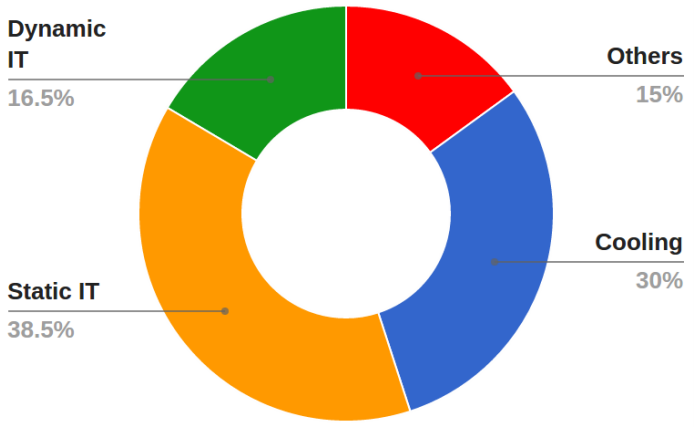
\includegraphics[width=0.5\textwidth]{percConsumoDC}
    \caption{Data center power usage distribution}

\end{wrapfigure}



Notice that PUE is always higher than 1 because IT Energy is contained in Total Facility Energy.

The perfect PUE would be 1. In this case, all the energy consumed  by the IT - servers, storage, network equipment... - would be the entirety of the energy consumption. This would be the ideal situation and there are no DC with this effectiveness.

Figure \ref{fig:pue-average} represents the evolution of PUE in Google's DCs along the last eigth years. Google DCs are considered one of the most power effective DCs around the world since they have the lowest PUE.

\begin{figure}[h]
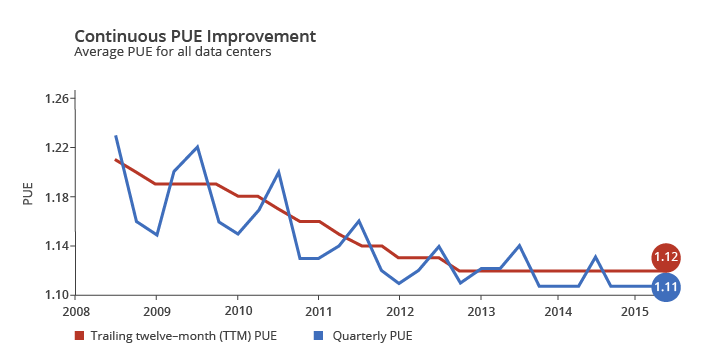
\includegraphics[scale= 0.5]{pue-average} % Podría poner[width=\linewidth]
\caption{PUE evolution of Google's DCs |\cite{puegrafica}}
\label{fig:pue-average} %Establece una etiqueta para la figura
\end{figure}
%\ref{fig:pue-average} % Devuelve el número de la figura
%\pageref{fig:pue-average} %Devuelve la página en la que está la figura

As can be seen in the plot, the PUE of Google DCS has progressively decrease year by year becoming almost 1 recently.

\subsubsection{Limitations of PUE \cite{ignacioPaper}} 

Even though, it seems a good idea to compare DCs depending on the PUE, PUE it is not the only comparison we should make talking about energy effectiveness.

As it was mentioned above, there are two contributors to the energy consumption: The server and the rest of the subsystems, and in this thesis we will focus on the consumption of the servers. According to the PUE formula, if the IT consumption is reduced, the PUE increases despite of the total energy consumption has been minimized and the DC has become more efficient.

Consequently, it can be said that PUE is a really important metric that has to be kept in mind, but it cannot be the single metric and must go with absolute metric such as consumption per server or consumption per full-load hour of each server. \cite{amer2013pue}

\subsection{Open Compute Project}

In April 2011, was announced the Open Compute Project (OCP). This project is led by Facebook with the aim of designing more efficient data centers. All the policies and designs introduced by the OCP have the same idea: making the DC a single environment where all the components - servers, building and software - can work at the same time and synchronized so that power-consumption and load share policies don't take decisions according to one component but to all the DC.

To achieve it, they share some specifications so that companies can create a new server based on the OCP specifications and, finally, the community can check if it really minimizes the energy-consumption and suggest some improvements. In this Bachelor Thesis an Intel version of the OCP server specification called Decathlete is used.

The reason why the OCP context has been chosen to work is that it is a four-years project in which some of the most important companies of the DC sector has worked. 

Finally, it is important to mention that OCP has some principles that share with this Bachelor Thesis. The most important points are the following ones:

\begin{itemize}
    \item First of all, it is based in Open Software and Hardware. Everyone can make and test its own changes without any restriction. This improves the speed at which the design upgrades.
    \item Second, OCP promotes a big research community. All new ideas are well-received at first. Then, the OCP decides which are the contributions that suit more the project and incorporates them to the main project.
    \item Thirdly, the main objective of the OCP is to create a new open standard so that several vendors could use the same standard.
\end{itemize}

\subsection{Green LSI framework}

Within this general framework, the Green LSI team also wants to participate in the optimization of the power-consumption of DC. Our work is focused on making the DC a single environment where all the components run at the same time. This synchronization is mainly targeted to reducing the power consumption. 

This thesis will be useful for the Green LSI researches for two reasons
:
\begin{itemize}
\item[$-$] Firstly, several lines of work of the GreenLSI has the aim of creating high level policies that do not have actuation support. It is a need of the group to create the tools to implement this policies in the group servers.

\item[$-$] Secondly, the results of this thesis can be applied to every server of the group so every line of work will have low-level support.
\end{itemize}
%%During this year, several works of the GreenLSI has been published.
%%Podría hablar de juan carlos y de marina como dos ejemplos del green lsi


%2015-ieee-cloudd = Marina
%2015-igsc = Marina
%2014-tpds = Zapater 
%Van los tres aquí



\subsection{Current Server-control Policies}
%Vasic N et al (2009) Making cluster applications energy-aware. In: Proc of automated ctrl for datacenters and clouds
%http://citeseerx.ist.psu.edu/viewdoc/download;jsessionid=0BAF373A528501F6B3ABF23028EBC947?doi=10.1.1.169.6157&rep=rep1&type=pdf
%46. Srikantaiah S et al (2008) Energy aware consolidation for cloud computing. In: Proc of HotPower
%http://research.microsoft.com/pubs/75408/srikantaiah_hotpower08.pdf

%Paper de alfonso
%Paper de ignacio
%Cualquier politica de actuación que solo hable de cómo manejar el consumo
As we can see in th paragraphs above, some policies at different levels inside the DC - servers, racks, hole DC - have been mentioned. One of them is at server level. Policies at server level need actuation support to implement them.

There are several research works focused on changing the configuration of a server to improve its performance, minimizing its consumption or a combination of both.

 
\begin{itemize}
    \item Research by Aransay et.al, in \cite{ignacioPaper} suggests a new algorithm to decide in which server should be allocated a new task in a data center. This algorithm recommends to use a Reputation System. Each server will have a reputation calculated using their CPU temperature and the most suitable server to allocate new workload will be established using this algorithm.

    \item In research by Felter et.al, \cite{Felter:2005:PAR:1088149.1088188}, they reduce peak power consumption by using workload-guided dynamic allocation of power among components. The idea is that not all the workloads need the same resources and these resources can be switched between power-saving and performance depending on the necessities.
    
    \item This document \cite{export:75408} suggests to consolidate applications in cloud-computing to reduce the energy consumption. This is because when an application needs low resources, the idle consumption predominate over the dynamic consumption so the server is not taking advantage of its resources. When applications are consolidated, this issue disappears.
    
    
\end{itemize}

    





\clearpage
\section{Multi-level actuation analysis}

Continuing with the line of argument, we consider four actuation levels. The idea is to analyze actuations that can be implemented in each level. The goal is to control all the subsystems at the highest level possible - user space level - as is the one that will allow to extend the policy implementations in more server models.

Most of the subsystems can be configured thought several levels of actuation, so a brief explanation of what is the difference between each level is been required.

\subsubsection{A) User-space level}

A modern computer operating system usually segregates virtual memory into kernel space and user space. Kernel space is strictly reserved for running a privileged operating system kernel, kernel extensions, and most device drivers. In contrast, user space is the memory area where application software and some drivers execute.

For this reason, in this thesis, any script or program executed by the user in the terminal has been named a user space tool. Examples of user level actuation are enabling and disabling CPUs and DVFS.

\subsubsection{B) Kernel level}

In contrast, kernel space implies changing configuration at lower level. It is useful to change some configurations that cannot be changed when the operating system is up.

In this case, to hotplug memories, some parts of the memory have to be configured as movable, in order to be able to disconnect them. This task is performed using kernel parameters.

\subsubsection{C) BIOS level}

BIOS is a type of firmware used during the booting process. The BIOS firmware is built into personal computers (PCs), and it is the first software they run when they are turned on. The fundamental purposes of the BIOS are to initialize and test the system hardware components, and to load a boot loader or an operating system from a mass memory device. 

But the BIOS also provides an abstraction layer for the hardware that enables the user to set some parameters related to the the hardware.

The server used in this thesis supports some settings to control the fan speed. User can set an RPM offset that makes fans run faster than they should. Offset must be a positive value.

\subsubsection{D) Service Processor}

This server has a service processor which controls some tasks that are usually of the Baseboard Management Controller.

This is very important for a server because, for example, it allows the server to be switched off when it is not used and then, just with a control signal sent by the internal service processor, to be switched on. During this period, the only contributor to the power consumption is the service processor and its consumption is minimum compared with the total consumption of the server. However, you need to take into account the time taken to turn the server on and off.

However it also controls everything related to the fan subsystem. The reason is that refrigeration is essential for the proper functioning of the server. If for any reason, the main server disconnects - for example, because of an elevated temperature - fans would stop running.

Consequently, it is necessary to contol the fan speed through the service processor.







\section{Server subsystems analysis}

The OCP has defined a specification for a server that can be used in a DC. This is the Decathlete specification. Intel, based on the Decathlete specification, has created the Intel S2600GZ server. Therefore, in this thesis, the server that is being used is an Intel S2600GZ server. \cite{serverSpecif} \cite{serverGuide}

\begin{figure}[H]
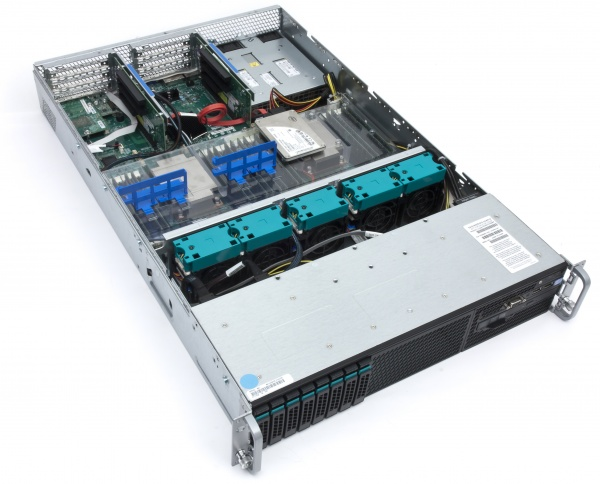
\includegraphics[scale= 0.5]{intel-r2000-s2600gz-server} % Podría poner[width=\linewidth]
\caption{Intel s2600GZ server.}
\label{fig:decathlete} %Establece una etiqueta para la figura
\end{figure}

Next, a brief information about the CPU, Fans, Hard drives and Memories will be explained in order to establish the scenario in which the thesis will developed. For each subsystem we will analyze the impact on overall power consumption and the control knobs available.

The hardware configuration of the Decathlete server in the Green LSI is not completely full. The number of components supported and those mounted in the server are detailed in Table \ref{tab:components}.

\begin{table}[H]
\begin{center}
\begin{tabular}{p{6cm} p{3cm} p{3cm}}
  \hline
  %\multicolumn{2}{c}{Components supported by the server}
  Components & Supported & Green LSI \\
  \hline
  Number of processors & 2 & 1 \\
  Number of DIMMS & 24 & 8 \\
  Number of Fans & 5 & 5 \\
  Number of power sources & 2 & 2 \\
  \hline
\end{tabular}
\end{center}
\caption{Components of the Green LSI s2600GZ server.}
\label{tab:components}
\end{table}

Therefore  according to previous work in the Green LSI team, the major part of the consumption comes from four contributors, the total consumption of the server can be divided into the following components:

\begin{equation*}
P_{TOTAL} = P_{CPU} + P_{MEMS} + P_{FANS} + P_{DISKS} + P_{OTHERS}
\end{equation*}

Where each of the terms are the power consumption of each of most important contributors to the total amount and OTHERS brings together the consumption of the rest of the components of the server - i.e.service processor, sensors, BMC, etc. - whose contributions can be considered negligible.

\begin{wrapfigure}{l}{0.5\textwidth}
    \centering
    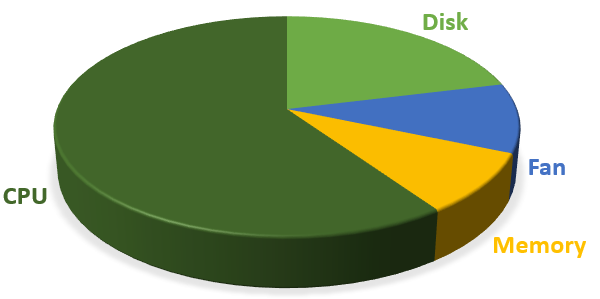
\includegraphics[width=0.5\textwidth]{totCons2}
    \caption{Average Decathlete's power consumption breakdown}
    \label{fig:totCons} %Establece una etiqueta para la figura
\end{wrapfigure}

Figure \ref{fig:totCons}~represents the breakdown of the main power consumption contributors of the server

This is the reason why the key data of their consumption will be studied down below.


\ \\ \ \\ \ \\ \ \\ \ \\
    \subsection{CPU}
    
    
    
    
    The Intel S2600GZ processor is an Intel® Xeon® Processor E5-2620 \cite{procDatasheet1} \cite{procDatasheet2} which has the specifications of Table \ref{tab:cpu_spec}.
    
\begin{table}[H]
\begin{center}
\begin{tabular}{p{6cm} p{3cm}}
  \hline
  \bf Number of cores & 6 \\
  \bf Number of threads & 12  \\
  \bf Processor base frequency & 2 GHz  \\
  \bf Range of scaling frequencies & 1.2 - 2.0 GHz. \\
  \bf Power & 85 W \\
  \hline
\end{tabular}
\end{center}
\caption{Specifications of the Intel® Xeon® Processor E5-2620. \cite{procTabla}}
\label{tab:cpu_spec}
\end{table}
%http://www.intel.com/content/www/us/en/processors/xeon/xeon-e5-brief.html

\begin{figure}[H]
\begin{center}
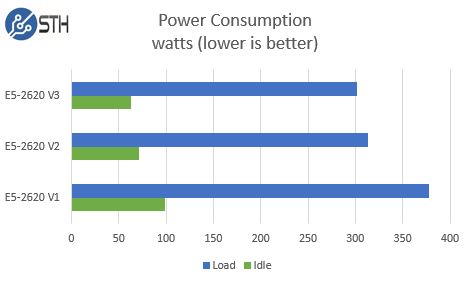
\includegraphics[scale= 1]{Intel-Xeon-E5-2620-V1-V2-V3-Power-Consumption} % Podría poner[width=\linewidth]
\caption{Power consumption of the Intel Processor \cite{procGrafica}}
\label{fig:Intel-Xeon-E5-2620-V1-V2-V3-Power-Consumption}
\end{center}
\end{figure}
%http://www.servethehome.com/dual-intel-xeon-e5-2620-v1-v2-v3-compared/

The breakdown of the power consumption of the CPU is the following:

\begin{equation*}
P_{CPU} = P_{CPU_{idle}} + P_{CPU_{leakage}} + P_{CPU_{dyn}} 
\end{equation*}
where:
\begin{itemize}
    \item[$-$] $P_{CPU_{idle}}$ is the consumption of the CPU when the server is not executing any load.
    \item[$-$] $P_{CPU_{leakage}}$ is the consumption associated with the leakage current in the CMOS. This consumption is exponential with the temperature.
    \item[$-$] $P_{CPU_{dyn}}$ is the consumption associated with the execution of the workload.
\end{itemize}


In this thesis, two actuation techniques associated with the processor will be checked.

\subsubsection{DVFS}

Dynamic Voltage and Frequency Scaling is a framework to change the frequency and/or operating voltage of a processor(s) based on system performance requirements at the given point of time.

Voltage scaling is achieved using voltage layer and regulator framework(driver). When frequency is scaled, voltage corresponding to the frequency is looked-up in the opp list. The device scale function requires the voltage layer to scale the device voltage to the target voltage.

The consumption saving is due to the switching power dissipated by a chip using static CMOS gates is 

\begin{equation*}
C * {V}^{2} * f
\end{equation*}
where:
\begin{itemize}
    \item[$-$] C is the capacitance being switched per clock cycle,
    \item[$-$] V is the supply voltage,
    \item[$-$] f is the switching frequency
\end{itemize}

so this part of the power consumption decreases quadratically with voltage. The formula is not exact however, as many modern chips are not implemented using 100$\%$ CMOS, but also use special memory circuits, dynamic logic such as domino logic, etc. Moreover, there is also a static leakage current, which has become more and more accentuated as feature sizes have become smaller (below 90 nanometres) and threshold levels lower.

\subsubsection{Turning ON-OFF CPUs}

Another technique that has been introduced in current servers and desktop computers is, when there are several CPUs, turning off some. This is necessary when the workload is too low or it cannot be spread into several cores.
%Esto ya se hace a nivel de BIOS

The idea is that, despite the CPU is not been used, power consumption due to leakage power is still there. This consumption emanates at a micro-level in transistors. Small amounts of currents are always flowing between the differently doped parts of the transistor. The magnitude of these currents depend on the state of the transistor, its dimensions, physical properties and sometimes temperature. The total amount of leakage currents tends to inflate for increasing temperature and decreasing transistor sizes.

This contribution is not as important as others, but it is easier to implement. In fact, there are some current policies based on this technique in the newest processors of the market. 

%%NO ES LO MISMO DISABLING QUE TURNING OFF

In this thesis, the idea has been disabling some CPU threads in order to study if the minimization of the power consumption balances out with the reduction of the computing power. This point will be developed in the next chapter.
%Insertar tabla






    \subsection{Fans}
    
    The server uses five fans of the company Nidec Corporation. The current configuration of the servers makes impossible to turn off one of the fans so they consume, according to the datasheet, 3.84 (W) per fan when they are at 4500 RPM. As there are five fans, the totally of fans consume 19.2 (W).
    
    \begin{comment}
    Additionally, related to the revolutions per minute (RPM) they can achieve, they have a maximum and a minimum cap:
    
\begin{itemize}
    \item[$-$] All the fans have a minimum RPM which is 6000 RPM. Regardless of the status of the server - idle, full-load, middle-load - fans cannot run at a lower speed.
    \item[$-$] The maximum speed that fans can achieve is 12.500 RPM which is an
    information obtained from the datasheet.
\end{itemize}
    \end{comment}


If any fan sensor or software detects that there is a failure or that there is not enough information to be sure that there is no failure, fans immediately start to run at full speed. Additionally, when one of the Hot-swap fans is removed to install another one, the time elapsed in which there are only four fans, they work at full speed, too.

\subsubsection{Reducing Fan speed}

%% Debería hablar de esto:
%%http://blog.stuffedcow.net/2012/10/intel32nm-22nm-core-i5-comparison/
%% Punto ideal de temperatura y consumo

Another way of reducing the energy consumption is reducing the air flow entered by the fans inside the server. According to the previous Green LSI study, DCs are over-refrigerated in some cases inducing a consumption expenditure that is not necessary.

The idea would be to study the impact of reducing the air flow - always being aware of compromise any server component. The consumption impact will depend on three variables: Density of the air, area of the fan and the air flow the fan moves.

According to this fact, the power consumed by a fan will respond as follows:
\begin{equation*}\label{eq:1}
Power\ = \frac{1}{2} * \rho * A * {V}^{3}
\end{equation*}
where:
\begin{itemize}
    \item[$-$] $\rho$ is the density of the air,
    \item[$-$] A is the area of the fan which is related to the size,
    \item[$-$] V is the air velocity
\end{itemize}

As the relation between energy and power is:
\begin{equation*}\label{eq:2}
Energy  = Power * Time
\end{equation*}

the relation between the air flow and the energy will be:
\begin{equation*}\label{eq:3}
Air\ flow\ \ \ \ is\ proportional\ to\ \ \ \ \ \sqrt[3] {Energy}
\end{equation*}

The conclusion is that this can be an important point to develop due to the fact that there is a chance that there is a considerable amount power saved. 

\begin{figure}[H]
\begin{center}
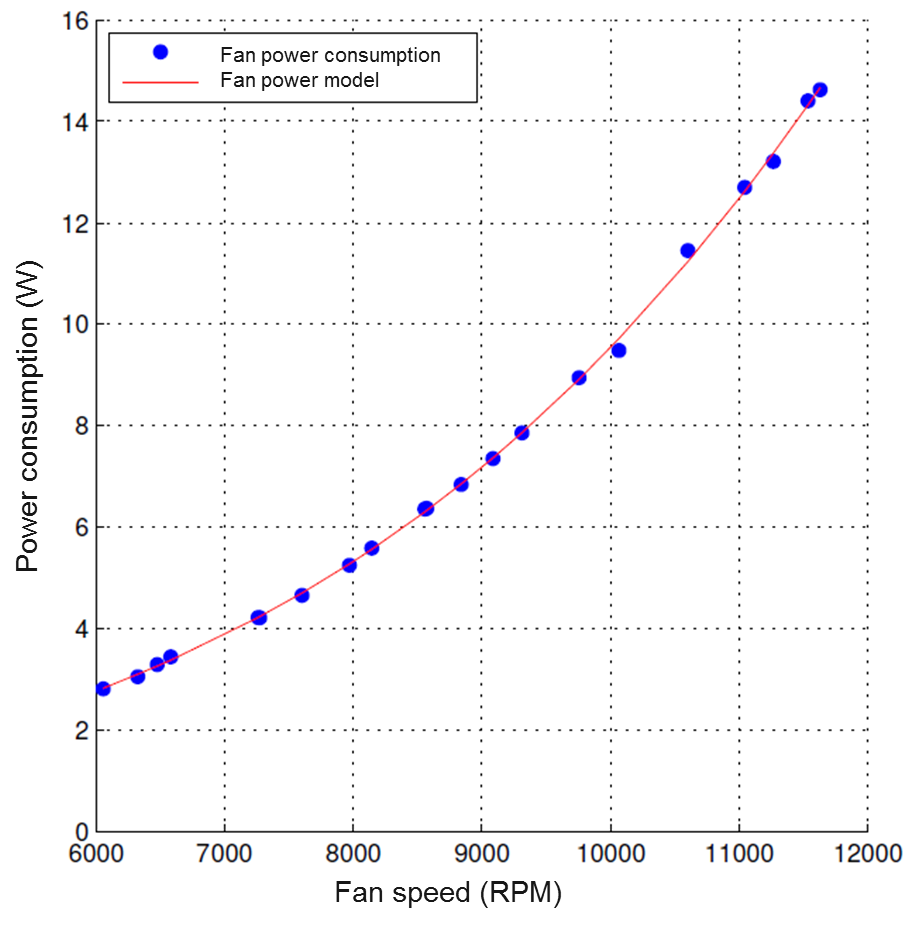
\includegraphics[scale= 0.7]{fan_speed3} % Podría poner[width=\linewidth]
\caption{Power spent depending of the RPM of the fan (~ Air Flow) in a generic server}
\label{fig:fan_speed} %Establece una etiqueta para la figura
\end{center}
\end{figure}
% Esto viene de https://www.usenix.org/legacy/event/hotpower08/tech/full_papers/tolia/tolia_html/index.html





    
    \subsection{Hard drives}
    
%http://www.seagate.com/www-content/product-content/constellation-fam/constellation/constellation-2/en-us/docs/constellation2-fips-ds1719-4-1207us.pdf

The server has four hard drives. The hard drives are designed by Seagate and the model is Constellation 2 \cite{diskDatasheet}. They have 1 TB of storage and use SAS as communication protocol.
    
\begin{table}[H]
\begin{center}
\begin{tabular}{p{8cm} p{3cm}}
  \hline
  \bf Idle power & 3.85 W \\
  \bf Typical Operating, Random Read & 6.4 W \\
  \bf Power Supply Requirements & +12V and +5V  \\
  \bf PowerChoice Technology & As low as 1.87 W  \\ 
  \hline
\end{tabular}
\end{center}
\caption{Specifications of the Seagate Constellation.2 SAS 1TB}
\label{tab:disk_spec}
\end{table}
    
Since there are used four hard drives, the consumption of the table has to be multiplied by four, remaining the total power consumption:
\begin{table}[H]
\begin{center}
\begin{tabular}{p{8cm} p{3cm}}
  \hline
  \bf Idle power & $3.85 * 4 = 15.4 W$ \\
  \bf Typical Operating, Random Read & $6.4 * 4 = 25.6 W$ \\
  \hline
\end{tabular}
\end{center}
\caption{RAID consumption Green LSI Decathlete}
\label{tab:disk_spec2}
\end{table}
    
    \subsection{Memory}
    
%% http://www.kingston.com/dataSheets/KVR16E11K4_32.pdf

Memories are from the model KVR16E11K4/32 from Kingston company \cite{memoryDatasheet}. In total, there are 32 GB of memory installed in the Decathlete, so there are eight modules of 4 GB each. The part of the information of the datasheet that is important for the thesis is the one presented in Table \ref{tab:mem_spec}

\begin{table}[H]
\begin{center}
\begin{tabular}{p{8cm} p{5cm}}
  \hline
  \bf Maximum Operating Power &  2.902 W (per module) \\
  \bf Total Maximum Operating Power & $2.902 * 8 = 23.21 W$ \\
  \hline
\end{tabular}
\end{center}
\caption{Memories consumption of the server}
\label{tab:mem_spec}
\end{table}

\subsubsection{Memories hotplugging}

Memories hotplugging is the same idea as turning on-off cpus. As it has been shown in the section above, memories consume around a quarter of all consumption of the server in idle status. This is the reason the memories have been selected to be studied.

Sometimes, the processes that are being executed in the server are not limited by the memories and they are being underused. In this cases, it would be interesting to shut down some memories so that server could save some energy.

This technique is not so widespread as turning off CPUs due to the fact that all the data allocated in that section of the memory must be moved to other section before turning the memory off. It is not so obvious to know exactly where the information is.

Due to the lack of an specific tool to perform this task, the procedure to achieve this goal will be detailed in Chapter 3.
%%\input{Chapter33}
\section{Monitoring and evaluation metrics}

In order to test our control techniques and to study the results in terms of energy, we present the monitory setup and describe the metrics we will use through this thesis.

\subsubsection{A) Monitory setup}

Monitoring setup is used to test if control techniques work.

\emph{Graphite}

Graphite is a highly scalable real-time graphing system. As a user, you write an application that collects numeric time-series data that you are interested in graphing, and send it to Graphite's processing backend, carbon, which stores the data in Graphite's specialized database. The data can then be visualized through graphite's web interfaces. 

Using Graphite, the following data can be analyzed:

\begin{itemize}
    \item[$-$] Server Power (For every component or subsystem).
    \item[$-$] Fanspeed.
    \item[$-$] CPU frequency.
    \item[$-$] Temperature.

\end{itemize}

\emph{Hardware counters}

Workload parameters can be obtained using hardware counters. Hardware performance counters are a set of special-purpose registers built into modern microprocessors to store the counts of hardware-related activities within computer systems.

There are a lot of counters, but in this thesis, only the count of clock cycles (CPU\_CLK\_UNHALTED), the count of instructions of the cpu (INST\_RETIRED) and the count of the last level cache misses (LLC\_MISSES) will be analyzed. Previous work of the Green LSI demonstrates that these are highly correlated with energy.

Performance counters are not displayed in Graphite already, but they are planned to be shown in future. One of the lines of work of the Green LSI is to make Graphite the big  and centralized monitoring system of every server of the team.


\subsubsection{B) Metrics}
\emph{Power}

Power does not depend on the time, so this metric cannot give us the amount of energy consumed. However, maybe a policy is very good at saving energy, but generates power demand peaks that cannot be assumed by the facility. This is why this metric is analyzed.

\emph{Energy}

Energy is also monitored because it represents the total amount of power consumption of a workload. It is directly related to costs. As energy is the result of multiplying the power by the time, the same workload will consume the same energy if consume high power in a reduced time or vice versa. This is the reason why not only the power is studied, but also the energy.

\emph{EDP}

EDP is the result of multiplying the energy consumed by the time in which it is performing the execution.
\begin{equation*}
EDP = ENERGY * TIME = POWER * {TIME}^{2}
\end{equation*}
The idea is that this metric allows us, using a single parameter, to detect quickly which configurations consume too much energy or time, because its EDP will be too high. Those test with similar EDP will have the same $energy * time$ product, and the decision about on what to prioritize - energy saving or performance -  should be made with other metrics.

This metric compares time and energy equally. This means that doubling time or energy will penalize in the same way the EDP. However, there are other metrics like ED2P or EDnP that penalize doubling the delay time versus the energy consumption, because they have the time in second power. 
%% http://link.springer.com/chapter/10.1007/978-1-4471-4492-2_8
%%Date: 05 Sep 2012
%%Energy Delay Product
%%James H. Laros III, Kevin Pedretti, Suzanne M. Kelly, Wei Shu, Kurt Ferreira, John %%Vandyke, Courtenay Vaughan

\emph{Performance}

However, power and its combinations are not the only point to take care about.The reason why time is so important for a data center is that it measures how a power saving policy delays the completion time of the benchmark. 

Given that a data center is supposed to be continuously computing workload, if a data center does not consider the performance apart from the energy consumption, the delay of processing can exceed the maximum allowed.
 
\emph{Counters}

Combining parameters, the \emph{number of instructions executed per cycle of clock} will be measured. This measure indicates how fast the processor can calculate the program that is being executed. It is proportional to the consumption of the processor.

% AQuí dedicaría un párrafo a explicar detenidamente qué es cpu intensivbe y memory intensive

The reason of this level of detail is that not all the benchmarks are CPU intensive. Those which are memory intensive spend too much time accessing to the memory but they do not need as much CPU performance as CPU intensive to execute instructions. This parameter will help us also to divide workloads into several types for several different policies.

The other parameter which is useful for this thesis is the \emph{number of last level cache misses}. A CPU cache is a cache used by the central processing unit (CPU) of a computer to reduce the average time to access to data from the main memory. This cache is a smaller and faster memory which stores copies of the data which are more frequently used.

Furthermore, a cache miss refers to a failed attempt to read or write a piece of data in the cache, which results in a main memory access with much longer latency. It may be important to be able to detect this type of workload and to operate it with a different policy.

\clearpage

\section{Proposed Actuation Techniques}

In this section, the methodology and steps followed to achieve the reduction of the power consumption will be detailed for each power management technique. There are two goals for this section: make possible to change the configuration of the server and see how this actuation saves energy.

\subsection{DVFS}

DVFS consists on changing the CPU frequency in order to save power. The saving is due to the higher frequency the processor works, the more current the transistors use. This is more detailed is previous section.

\subsubsection{CPUfreq}

To achieve the frequency scaling task it is used CPUfreq which is a Linux kernel framework that monitors the performance requirements of a processor(s) and takes decisions to increase or decrease operating frequency in order to save power and/or reduce leakage power.

As CPUfreq is a user-space Linux framework, which is the highest level, other actuation techniques for other levels of abstraction are not studied. 

The frequency management works this way while using CPUfreq. When you configure CPUfreq in a server you have to specify a \emph{Policy}. A policy is a combination of two parts: \emph{frequency limits} $(policy\-\>\{min,max\})$ plus CPUfreq \emph{governor} to be used. In this case, the frequency limits are 1.2GHz until 2.0GHz. The governor possibilities are: userspace, ondemand or performance.

The governor is who decides what frequency should be used. To do this task, depending on which governor you choose, it changes the frequency within the values of the limit of the policy. There are some default governors and every user can define its owns.

Default governors are quite simple. Here is the explanation of them:

\begin{tabular}{ p{2.3cm} p{10.2cm}}
  \bf Userspace & Allows the user, or any userspace program running with UID "root", to set the CPU to a specific frequency by making a sysfs file "scaling\_setspeed" available in the CPU-device
directory. \\ \\
  \bf Performance & Sets the CPU statically to the highest frequency within the borders of scaling\_min\_freq and scaling\_max\_freq. \\ \\
  \bf Ondemand & Sets the CPU frequency depending on the current usage. To do this the CPU must have the capability to switch the frequency very quickly. The frequency always jump between the min and max frequency value. When there is any load on the CPU, the frequency jumps to max speed.\\ \\
\end{tabular}

By default, any time the server reboots, it turns on with the "ondemand" governor, so it is necessary to switch to userspace in order to make some tests.

There are some only-readable files that give important information to use DVFS:

\begin{tabular}{ p{2.3cm} p{10.2cm}}
  \bf scaling\_ available\_ frequencies & This file contains the available frequencies in which the server can work. In this case, our server has the following frequencies: 1.2Ghz, 1.3GHz, 1.4GHz, 1.5GHz, 1.6GHz, 1.7GHz, 1.8GHz, 1.9GHz, 2.0GHz, 2.001GHz \\ \\
  \bf scaling\_ available\_ governors &  This file contains the available governors for this server. In this case, our server has the following governors: Userspace, ondemand and performance. \\ \\
    \bf cpuinfo\_ cur\_ freq &  This file contains the actual frequency of the server obtained from the hardware. This file is useful to know if the script of changing the frequency has finished correctly.  \\ \\
  \bf scaling\_ curr\_ frequency &  This is	the frequency the kernel thinks the CPU runs at. It is important not confuse  this one and the cpuinfo\_curr\_freq. \\
\end{tabular}

\subsubsection{Benchmarks}

There have been used four different types of Benchmark in this thesis. The choice had the aim of covering the largest range of possibilities with the smallest number of tests. \cite{specCPU}

\emph{SPEC CPU}

To perform this Benchmarks, SPEC CPU has been used. SPEC CPU is a suite designed to provide a comparative measure of compute-intensive performance across the widest practical range of hardware using workloads developed from real user applications.

It has over 30 benchmarks but in this thesis only four of them will be used. The choice includes two integer benchmarks - Perlbench and Mcf - and two floating point benchmarks - Calculix and Lbm. 
Furthermore, it also has been chosen depending on if they are cpu intensive or memory intensive. With this classification, Perlbench and Calculix are CPU intensive and Lbm and Mcf are Memory intensive.

\begin{tabular}{ c| cc}
  \bf  & CPU Intensive & Memory Intensive \\
  \hline
  \bf Integer  & Pearlbench & Mcf \\
  \bf Floating Point  & Calculix & Lbm \\
\end{tabular}

\ \\ \ \\ \ \\
To execute the script it is only needed to put the following parameters: the number of the cpu you want to change the frequency and the frequency you want to change to. Given that this tool does not allows the user to change several cpu`s frequencies at the same time, it has been developed an script to create a new higher-level layer that implements this feature.

The analysis consisted of loading some SPEC benchmarks in several server environments and measuring some stats from the server. In the DVFS test, all the combinations of the following statistics will be tested:

\begin{tabular}{ c| cccc}
  \bf Frequency & 1200000 & 1500000 & 1700000 & 2000100 \\
  \bf Benchmark & Perlbench & Calculix  & Lbm & Mcf \\
  \bf Nº Copies & 1 & 3       & 6  & 12\\
\end{tabular}


All the possible combinations of frequency, benchmark and number of copies of the same benchmark in order to analyze the time spent and the power, energy and EDP consumption of the server.


\subsubsection{Turbo Boost}

Intel® Turbo Boost Technology accelerates processor and graphics performance for peak loads, automatically allowing processor cores to run faster than the rated operating frequency if they’re operating below power, current, and temperature specification limits. The amount of time the processor spends in that state depends on the workload and operating environment.

In this thesis, the turbo boost frequency is analyzed to calculate how much energy this feature consumes. Much more consumption is expected at this frequency than at a lower frequency given that the server is running at 100\% of its power.



\subsection{Disabling and enabling threads of the CPU}

This is another way of saving energy in a server. The idea is that if a threads of the CPU is not necessary, it would be better to turn it off to save energy.

\emph{C-States}

Advanced Configuration and Power Interface (ACPI) is an open specification created to uniform all the techniques focused on managing power consumption, among other things.

In this specification, C-states are defined. A C-state is a core power state that defines the degree at which the processor is "sleeping". C0 corresponds to the normal state in which the processor can achieve the 100\% of its capacity and Cn corresponds to several power states. Not all the processors can change to all states because some of them are defined for specific processors.

The decision about in which power state must be the processor corresponds to the Operating System Directed Power Management. It does it transparently for the user and the user cannot manage in which C state is going to be the processor. The only thing the user can decide is, for each C-state, if the OS can switch to this C-state, but not when or how.

This is the reason why in this thesis C-states have not been managed.

\emph{Disabling cores}


\begin{wrapfigure}{r}{0.5\textwidth}
    \centering
    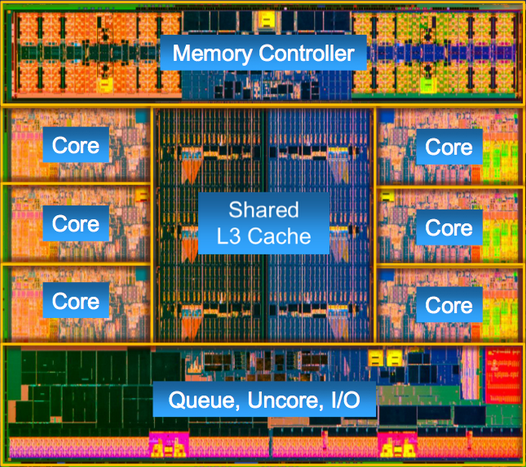
\includegraphics[width=0.5\textwidth]{esqProc}
    \caption{Schema of a typical 6 core processor}
    \label{fig:esqProc} %Establece una etiqueta para la figura
\end{wrapfigure}

In this thesis, what is has been done is to disable threads. Thanks to this processor architecture, the processor is divided in 6 hardware cores which are subdivided in 2 threads or logic cores. Figure \ref{fig:esqProc} represents the schema of the processor.

As the OS can manage the configuration of each thread separately, the main objective has been to disable them in order to understand how the number of threads is related to the performance of the server. Disabling threads leads to two reactions: the power consumption decreases, but it also decreases the performance of the cpu. Disabling threads will only reduce the performance because disabling is just not allowing a process to be executed by this processor.

The idea is that by disabling threads we can analyze if the time a benchmark elapse grows and if it increases the energy consumed by the benchmark. 

\subsubsection{chcpu}

To carry out this undertaking it has been used chcpu which is a command part of the util-linux package. Chcpu can modify the state of CPUs. It can enable or disable CPUs, scan for new CPUs, change the CPU dispatching mode of the underlying hyper-visor, and request CPUs from the hyper-visor (configure) or return CPUs to the hyper-visor (deconfigure).

In this case, only the function of disabling and enabling cpus has been used.

\begin{lstlisting}[language=Bash]
chcpu disable <Core number [1...11]>
\end{lstlisting}

Notice that core 0 cannot be disabled because it is the master core where the OS runs.

In the next chapter, the analysis about this actuation technique will be detailed.

\subsection{Off-lining Memories}

The main goal of this technique is to off-line memory modules seeking for a power consumption reduction.

In the last memory hotplug update, there is a folder structure used to see and change the status of the memory blocks. There are three important files in the hot-plug/hot-off-lining process:


\begin{tabular}{ p{2.4cm} p{10.5cm}}
  \bf State & When reading, it contains the online/offline state and when writing, it allows to change between online, offline, online kernel $-$ At the same time this memory block is online , it is configured as kernelcore $-$ and online movable $-$ At the same time this memory block is online, it is configured as movablecore \\ \\
  \bf Removable &  Indicates if the memory block is removable or not. It contains an 1 if is removable and a 0 if it is not \\ \\
  \bf Valid\_zones &Specifics the states the memory block can switch to\\
\end{tabular}


As we will just explain how removing memories work, we will talk about Hot-Remove instead of Hot-plug. In order to properly switch off a DIMM, there are three phases in Memory Hot-Remove:

\begin{description}
 \item[Step 1] Movable Memory Set
 \item[Step 2] Logical Memory Remove
 \item[Step 3] Physical Memory Remove. (To be developed)
\end{description}

\subsubsection{Movable Memory Set}

This phase intends to make the whole memory block be unused. The problem is that memory offline can fail if the memory block includes memory which cannot be freed. Memory that can be freed is that whose all pages can be migrated to other memory block.

To understand how memory permissions work, we need to explain all memory migratable configurations. Memory modules can be configured as kernelcore, movablecore and not-configured.

\begin{itemize}
    \item[$-$] Parts of the memory that are configured as \emph{kernelcore} are reserved for processes of the kernel only. These pages cannot be moved, so this parts cannot be migratable and, in short, removed.
    \item[$-$] Parts of the memory that are configured as \emph{movablecore} are reserved for processes that can be reallocated in other memory modules. This is the amount of memory we can be sure we will be able to logically remove.
    \item[$-$] Finally, the memory does not have to be configured.
\end{itemize}

This configuration must be made through a booting option of the kernel in the GRUB stage.
\subsubsection{Actuation technique: GRUB}

GNU GRUB is a boot loader package from the GNU Project, which allows a user the choice to boot one of the multiple operating systems installed on a computer or select a specific kernel configuration available on a particular operating system's partitions.

So, when grub starts, a movablecore or kernelcore has to be set in order to select the amount of memory wanted to be migratable and not-migratable.

To test if this can be modified, we followed the next instructions:

\begin{lstlisting}[language=Bash]
#When grub starts, press "e" to enter in GRUB configuration.
#Add the memory option at the end of the following line:

linux /boot/vmlinuz-linux <More boot options>

#Finally, press "b" to boot with the new parameters.
\end{lstlisting}

This only makes changes for this time, if the changes must be permanent, this file has to be modified:

\begin{lstlisting}[language=Bash]
# In file /etc/default/grub add
# one or both of the following lines:

KERNELCORE = <Amount of memory in GB>
MOVABLECORE = <Amount of memory in GB>

#Finally, execute:

grub-mkconfig -o /boot/grub/grub.cfg

\end{lstlisting}



The problem is that when the OS starts, there is no information about which memory belongs to movable or to not movable.

\subsubsection{Logical Memory Remove}

In the second step, using the sysfs interface just have to change the "state" file to offline and if the first step was correctly completed, this step must be ok.

When a memory is logically removed, no task can allocate information in this memory block until it is plugged again. At first, there is no sign that just logical remove saves power. The technique saves power if when a memory is off-lined, power is saved.

It is expected that physical memory remove will save energy when it is implemented.

\subsubsection{Conclusion}

During this thesis, several attempts of hot-removing memories has been made. Despite, it is not possible to reduce the power consumption generated by the memories.

Thanks to this work, some gaps have been identified in this issue. First of all, memories hot removing is not completely implemented at this moment. There is a lot of work pending to be done.

The server that the group has in its facilities does not have the latest version of centOS. Actually, it has the CentOS release 6.6 (Final). CentOS is currently in version 7.0. With this 6.6 version, configuration files are not the definitely ones and logical memories remove cannot be properly done.

Hopefully, some personal computers in the group has CentOS 7.0 installed. Using this computers, memories could be logically removed, but not physically removed. The issue comes from that memories can be disabled and the SO is notified of it, but then there is no way to know which physical module corresponds to the logical module, so the SO cannot turn it off.

\subsection{Changing fan speed}

Changing Fans Speed was one of the first goals of this thesis due to previous work showed that this could be a technique that could easily reduce a great amount of power consumption.

Despite the other subsystems are directly connected to the Baseboard Management Controller, fans are controlled by the Service Processor. \cite{serverSpecif}

The service processor is a separate, dedicated internal processor located on the motherboard of the server. It operates independently from the server’s CPU and operating system (OS), even if the CPU or OS is locked up or otherwise inaccessible.
%http://www.emersonnetworkpower.com/en-US/Latest-Thinking/Pages/avocent-thought-leadership-service-processor-management.aspx

The service processor monitors the server’s on-board instrumentation (temperature sensors, CPU status, fan speed, voltages), provides remote reset or power-cycle capabilities, enablse remote access to basic input/output system (BIOS) configuration or OS console information and is responsible for the fan speed control.

The difficulty of this task comes from the fact that the server uses a Service Processor to control the fan speed. Common \emph{Linux} speed control scripts modifies only the fan speed if it is controlled through the BMC, for this reason, they are not useful for this thesis.

The service processor uses an IPMI technology. For this reason, in this thesis is used ipmitool as the tool to control the service processor.

Ipmitool lets you manage Intelligent Platform Management Interface (IPMI) \cite{ipmiSpec} functions of either the local system, via a kernel device driver, or a remote system, using IPMI V1.5 and IPMI v2.0. In this case, it is used IPMI v2.0
%Enlace a las especificaciones de ipmi v2

The next step was to be able to change the speed through the \emph{BIOS}. BIOS have direct communication with the SP an is able to change the fan speed. The issue is that there is only one option which is to add a threshold to the current fan speed, but not reducing the speed what was the aim of the thesis. Previous work of the GreenLSI has modeled the behaviour of the fan consumption depending on the air flow.

Now, before explaining the third step, it is important to distinguish between two ways of introducing improvements into the server: the less invasive, which consists in adding a new abstraction layer that enables us to do whatever we want without modifying what it was already there - it can be both hardware or software - and the intrusive one which is to modify something that is already in the code or in the hardware.

The third attempt was related to analyze the code of the \emph{kernel} of the SP to find out how the SP decides the fan speed. The idea was to modify the code to allow us to change the speed wherever we want in some way. Despite all the code is available, it was not clear where the decision algorithm was so it cannot be changed.

Finally, the single option is to change it through \emph{IPMI} which allows the BMC and the SP to give parameters and information to each other.

Using IPMI \cite{serverConfigIPMI}, there were two processes that could had helped us in this task:

\begin{itemize}
    \item[$-$] Giving some raw commands:
\end{itemize}

This was the first idea of how to modify the fan speed using IPMI. There is a document that describes Facebook's Fan Speed Control (FSC) and its update methodology
The aim Facebook has writing this document is to standardize how the server management controller manages FSC parameters.

With this new commands, two points can be managed through ipmi. On the one hand, Pulse Width Modulation (PWM) can be set directly. To perform this feature, a raw command of this layout must be sent: 

\begin{lstlisting}[language=Bash]
impitool [options] raw 0x30 <PWM ID> <PWM value> 
            #0x30 allows us to send FSC commands.
\end{lstlisting}

On the other hand, Facebook provides some simple control or information algorithms that can be set as profile of the fans in order to control the fan speed or calculate related parameters. There are four algorithms divided into Linear and Non-Linear.

\begin{itemize}
    \item[$*$] \textbf{Linear. Temperature: }This set controls the fans speed depending of the temperature. If it exceeds a threshold value, fan speed increases. The algorithm outputs the pwm value in percentage.
    \item[$*$] \textbf{Linear. FAN RPM: }This set controls the average of Cubic Feet per Minute (CFM) that the fans move. As input it has the Fan rpm and outputs the CFM.
    \item[$*$] \textbf{Linear. Power: }This set calculates the relation between the power used by the fans and the PWM in which it is translated.
     \item[$*$] \textbf{Non-Linear. PID Controller: }PID is the acronymus of Proportional, Integral, Derivative (PID) controller which is a widely used control loop feedback mechanism. This is a non-linear algorithm that allows to control fan speed control. It is more complex than the others to be more exact.
\end{itemize}

To change this profiles, entering and exiting in update mode is required to the changes take effect.

Despite it is well documented by the specification of the Facebook's Decathlete server, it is not well implemented in the S2600GZ server from Intel, which is supposed to fulfill the Decathlet's specifications. That is why it cannot be tested in this thesis.

\begin{itemize}
    \item[$-$] Changing the threshold parameter
\end{itemize}

Finally, another way of changing the fan speed was tested. The SP uses several registers to determine if the temperature of the server is within the correct values or, by contrast, it is over the well-functioning range. The idea was to change this registers in order to make the server run the fans slower to see how the temperature and the performance changes.

\begin{lstlisting}[language=Bash]
ipmitool sensor thresh <sensor name> lower <lower 
    non-recovery value> <lower critical value> <lower
    non-critical value>

ipmitool sensor thresh <sensor name> upper <upper
    non-critical value> <upper critical value> <upper
    non-recovery value>
\end{lstlisting}

Seemingly, it is not well implemented. When one of this registers is changed, all the fans began to run at the maximum speed, 12 000 RPM and never reduce their speed despite there is no issue. We leave for future the debugging of this technique.

\subsubsection{Conclusion}

%Muy interesante esta página http://www.opencompute.org/wiki/Server/SpecsAndDesigns
As it is described in the document of the OCP \cite{fanspeed}, the Open Compute Project defined a new algorithm to manage fan speed of the servers. The 0.1 version of this algorithm was published in 2014. The problem is that a document from the OCP does not automatically generates a new release of the Intel Service Processor.

% Creo que es este firmware https://downloadcenter.intel.com/download/24617/Intel-Server-Board-S2600GZ-GL-Firmware-Update-for-IDA-and-OFU
In this case, the problem is similar to what occurs with memories hotplug. The version of the SP's kernel is not the latest one and it cannot be checked if the latest version has already implemented the algorithm published in the paper. To update to the latest version and to check if it works properly is to be done.


\subsection{Summary}

To sum up, here is a table with the studied levels for each subsystem. It is important to emphasise that the aim has been always to find a higher level solution.


\begin{table}[H]
\centering
\label{my-label}
\begin{tabular}{c|cccc}
LEVEL & MEMORIES & CPU Disabling & DVFS & FAN SPEED\\ %\cline{2-5}
\hline \\
User Space & \multirow{3}{*}{YES} & Implemented & Implemented & NO \\ \\
Kernel  &                   &  &  & NO \\ \\
BIOS &      Limited             &  &  & Offset only \\ \\
SP &                   &  &  & Firmware dependant \\ 
\end{tabular}
\caption{Summary of the possible actuation levels over Intel S2600GZ}
\end{table}

In memories subsystem, the solution is a combination of User-space and kernel levels.




\clearpage

\section{Experimental Evaluation}

In this section we detail the results obtained when testing our actuation techniques. As CPU power consumption is the major contributor to overall server power, for time reasons, we focus our experiments on the CPU subsystem.
\subsection{Main test}

To obtain some results in the next actuation techniques, a script to launch all the benchmarks has been executed in the server. This script executes all the selected benchmarks through all the possible energy-consumption configurations in order to obtain some metrics.

\begin{lstlisting}[language=Bash]
for frecuency in Frecuencies[@]; do
    change_cpu_freq -all
    sleep 1m
    for benchmark in Benchmarks[@]; do
        for numberCPUs in Cpus[@]; do
            disable_cpu <numberCPUs>
            for numberCopies in Copies[@]; do
                - Execute the Benchmark -
                sleep 5m
            done
        done
    done
done
\end{lstlisting}

As explained in chapter 4, 128 Benchmark-Configuration pairs were executed and the results will be analyzed in the following section.

\subsection{CPU and Memory intensive benchmarks}

Apart from analyzing how power consumption is reduced, it is also important to be able to detect when a benchmark is CPU or memory intensive. To do so, some counters help us.

As expected, Perlbench and Calculix have more "instructions per cycle" (IPC) than Mcf and Lbm. This is because memory intensive benchmarks have much more "Last Level Cache Misses" (LLC\_Misses). This issue makes the processor work slower because it has to wait until the thread access to the main memory to recover the data needed.

As we are running several copies of sequential benchmarks, as long as there is no contention, IPC and LLC can be used to cluster benchmarks into various categories. Moreover, this two metrics are not affected by the processor frequency. Thus, IPC and LLC depend on the benchmark being executed. For that reason, when a new workload is executed, its type can be easily detected and this can be an interesting point to start the design of a new policy.

Next figure shows the average IPC and LLC\_misses.

\begin{table}[H]
\begin{center}
\begin{tabular}{p{4cm} p{3cm} p{3cm}}
  \bf &  IPC & LLC Misses \\
  \bf Pearlbench & 1.76 & 3.68 $\cdot {10}^{8}$ \\
  \bf Calculix & 2.49 & 2.05 $\cdot {10}^{8}$\\
  \\
  \bf Lbm & 1.18 & 2.22 $\cdot {10}^{9}$\\
  \bf Mcf & 0.39 & 6.43 $\cdot {10}^{8}$\\
\end{tabular}
\end{center}
\caption{IPC and LLC misses for each benchmark}
\label{tab:ipcllc}
\end{table}

\begin{figure}[H]
\begin{center}
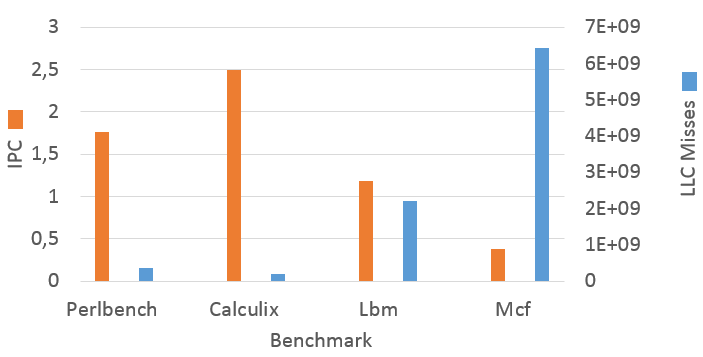
\includegraphics[scale= 0.80]{llcipc} % Podría poner[width=\linewidth]
\caption{IPC and LLC misses for each benchmark}
\label{fig:llcipc} %Establece una etiqueta para la figura
\end{center}
\end{figure}


\subsection{DVFS}

Now, DVFS consequences in power consumption will be analyzed. For the next figures, the value of CPU total consumption is used to compare all the benchmarks. It would be better to compare the Dynamic consumption of the cpu, but the values are not so accurate. The sensor that is installed in the Decathlete to measure the consumption of the server has a resolution of 4W. As some of the dynamic values are below 4W, this values will not be used in this comparison.

In some data centers there is a need to put a cap on maximum power, to ensure that the facility does not exceed the maximum power budget. In such cases, we may benefit from lowering frequency to save power. However, among the various configurations, we need to chose one that reduces. Based on this results, we could develop policies to set the frequency of servers depending on the particular workload to be executed.

To calculate the total consumption of the CPU, we have subtract the power consumption of the disks, memories and fans from the value of total consumption of the server. All this values have been obtained using Graphite, so they are all experiment results. The X axis contains each benchmark, while the Y axis shows the power consumption.

\begin{comment}
The X axis represents, using a code, each benchmark. The code can be interpreted this way:

Part1\_Part2\_Part3
\begin{itemize}
\item [$-$] Part1: This is the name of the type of the benchmark. As it was detailed in a previous section, there are four benchmarks: Perlbench, Calculix, Mcf and Lbm.
\item [$-$] Part2: This is the number of threads enabled. Possible values are 1, 3, 6 and 12
\item [$-$] Part3: This is the number of copies of the same benchmark executed at the same time. Possible values depend on the number of threads enabled.
\end{itemize}
\end{comment}

Figure \ref{fig:potenciaFreq} shows how power consumption depends on the frequency.


\begin{figure}[H]
\begin{center}
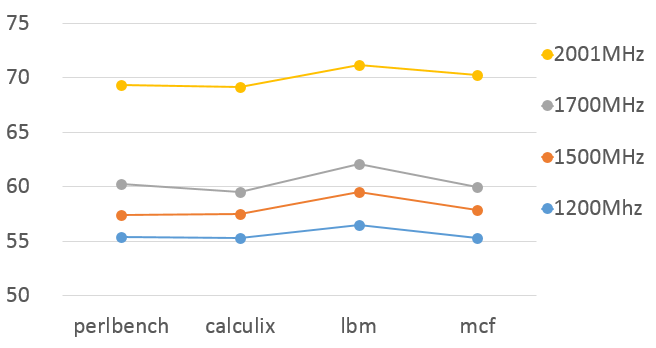
\includegraphics[scale= 0.65]{compPower2} % Podría poner[width=\linewidth]
\caption{Power consumption in Watts depending on the frequency}
\label{fig:potenciaFreq} %Establece una etiqueta para la figura
\end{center}
\end{figure}

Analyzing the results, it can be seen that power depends on the frequency. For the same benchmark, savings of almost 25\% can be achieved reducing the frequency from 2001MHz to 1200MHz. Of course, as power does not depend on the time elapsed, benchmarks cannot be only compared this way. For this reason, in Figure \ref{fig:edpFreq} the EDP of each benchmark is shown. To calculate the EDP, power has been multiplied by the second power of the time, which has been obtained thanks to a log saved during the execution of the script.

\begin{figure}[H]
\begin{center}
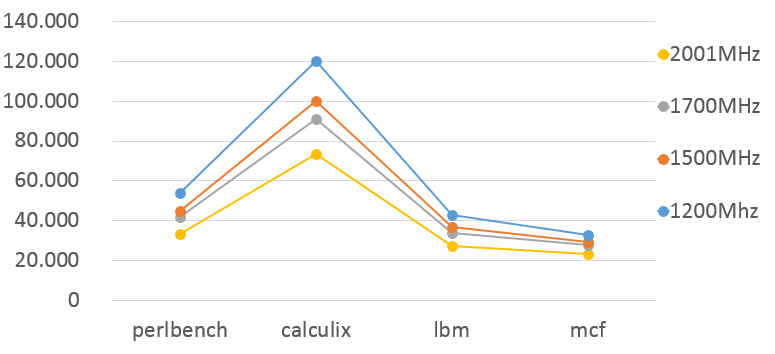
\includegraphics[scale= 0.6]{edp_Freq5} % Podría poner[width=\linewidth]
\caption{EDP of each benchmark depending on the Frequency}
\label{fig:edpFreq} %Establece una etiqueta para la figura
\end{center}
\end{figure}

In this Figure, changes can be seen when we consider the contribution of time to the metric. Despite the power consumption is lower, the time elapsed is higher so the EDP recommends to use the highest frequency. Energy plot is not shown given that its shape is similar to the EDP one, so it is not necessary.

According to the data obtained, it is experimentally demonstrated that the choice of the most suitable frequency depends on the aim to achieve. If the goal is to minimize the power consumption - reducing the power consumption peaks - it is better to reduce the frequency of the processor. If the goal is to maximize the performance and, therefore, minimize the energy consumption and the EDP, the most suitable solution is to run at higher frequencies.

Despite this level of detail cannot be represented in the plot, the gap between 2001MHz and the others is higher than the rest. The reason is that 2001Mhz is the Turbo Boost frequency. As it was explained in the DVFS section, at this frequency the processor has to do its best and this maximizes the contribution to the CPU power consumption.


It can be seen also in Figure \ref{fig:edpFreq} that not all the Benchmarks vary the same when the frequency changes. Those which are cpu intensive have a higher variation in it EDP. This is because cpu benchmarks depends only on how fast can the processor calculate. When the frequency is high the EDP is lower. However, in mcf and lbm benchmarks, the bottleneck is not for the processor, but for the time elapsed accessing to the main memory. For that reason, the EDP does not vary at all in them.


\subsection{Disabling Threads}

%%Aquí las cosas de comparar idle.

\emph{Analysis of the idle consumption}

Disabling threads has also given interesting results. First of all, it has been analyzed if disabling them could achieve savings in power consumption. As it is shown in Figure \ref{fig:cpuGraf}, which is a capture of Graphite, mean power consumption is constant when the number of threads changes.

In this capture, the same process as in the other tests has been followed. The server has been configured for 5 minutes in all the power consumption possible configurations. The plot represents the total consumption of the server in the Y axis, while the X axis represents the time.

\begin{figure}[H]
\begin{center}
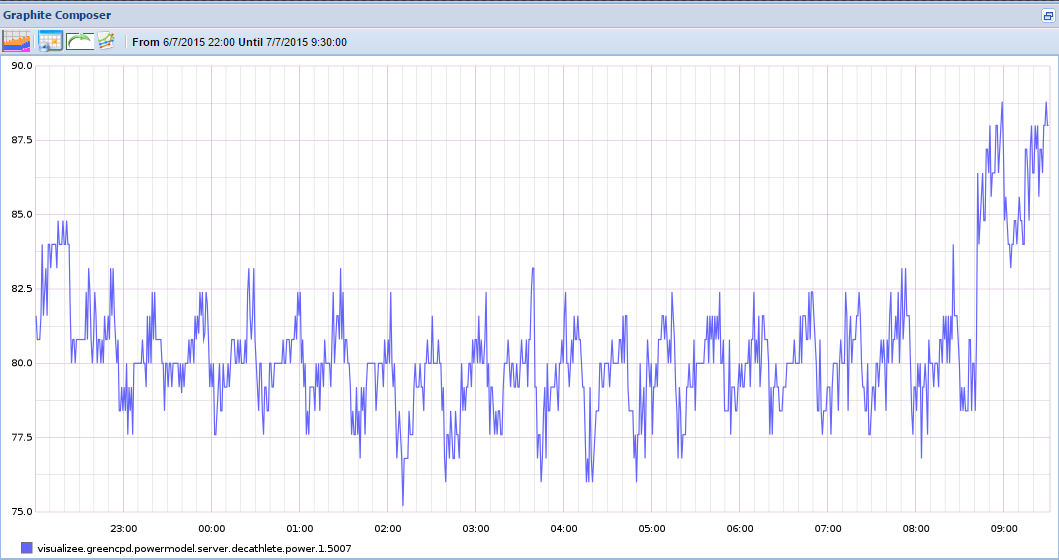
\includegraphics[scale= 0.52]{grafIDLE} % Podría poner[width=\linewidth]
\caption{Total server consumption depending on frequency and threads enabled}
\label{fig:cpuGraf} %Establece una etiqueta para la figura
\end{center}
\end{figure}

This means that even though we are disabling threads in user space, the change is not being implemented in lower levels, i.e. it is not directly supported by the Intel CPU drivers. In this sense, we observe no benefits in terms of power when disabling threads in idle load.

\ \\ 

\emph{Analysis of the consumption of a workload}
%%Aquí las cosas de comparar benchmarks

Apart from the test above, in which no benchmark was running, so as the idle power was similar to CPU and proportional to the total server power consumption, another test has been run. Now, the same test as in the DVFS section will be analyzed.

Despite we have not been able to turn off CPUs, threads have been disabled. This give us the opportunity to study the performance depending on the number of threads.

In Figure \ref{fig:timeProc} the performance of each benchmark will be analyzed. The time elapsed in each benchmark is represented in the Y axis and the X axis has each benchmark. 

\begin{comment}The benchmark code must be analyzed in the same way:

Part1\_Part2
\begin{itemize}
\item [$-$] Part1: This is the name of the type of the benchmark. As it was detailed in a previous section, there are four benchmarks: Perlbench, Calculix, Mcf and Lbm.
\item [$-$] Part2: This is the frequency at which the processor runs for this benchmark.
\end{itemize}
\end{comment}

\begin{figure}[H]
\begin{center}
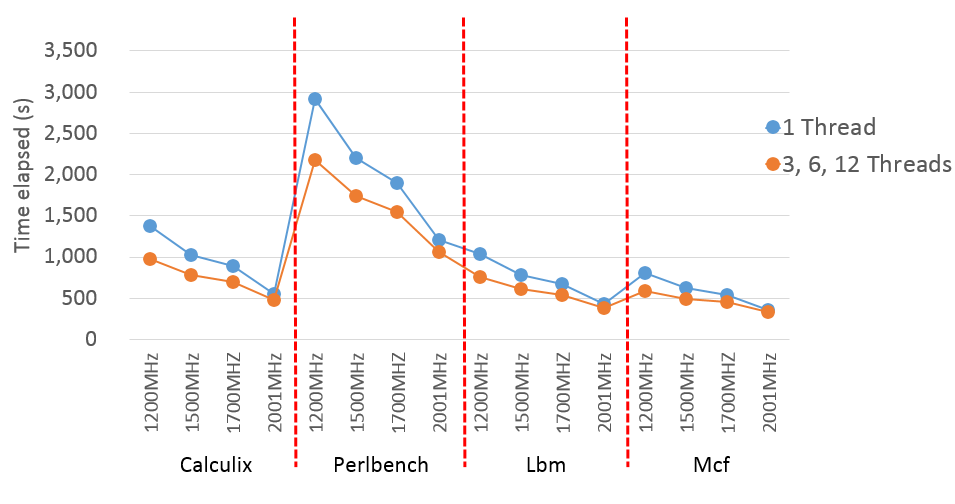
\includegraphics[scale= 0.6]{timeProc3} % Podría poner[width=\linewidth]
\caption{Time spent in each benchmark}
\label{fig:timeProc} %Establece una etiqueta para la figura
\end{center}
\end{figure}

As it can been seen in this figure, there are two different performances when disabling threads. When using only one core for one thread, the time elapsed grows. This is caused by two reasons: 

\begin{itemize}
\item [$-$] First, when using just one thread, all the processes must be executed in the same thread. This means that all OS processes have to share the processor resources with the benchmark. This issue caps the performance. When more that 1 thread is enabled, one of them can be exclusively used for the benchmark.

\item [$-$] Second, Hyper-threading which is the Intel's proprietary simultaneous multithreading (SMT) implementation. This technology makes the processor compute faster. 
\end{itemize}

The main function of hyper-threading is to increase the number of independent instructions in the pipeline; it takes advantage of superscalar architecture, in which multiple instructions operate on separate data in parallel. In addition, two or more processes can use the same resources: if resources for one process are not available, then another process can continue if its resources are available. This enables the server to make a better performance when using several threads.

\ 

CPU power consumption seems to remain the same. Figure \ref{fig:powerProc} represents the cpu total power consumption in Y axis for each Benchmark in X axis depending on the number con threads enabled. 

\begin{figure}[H]
\begin{center}
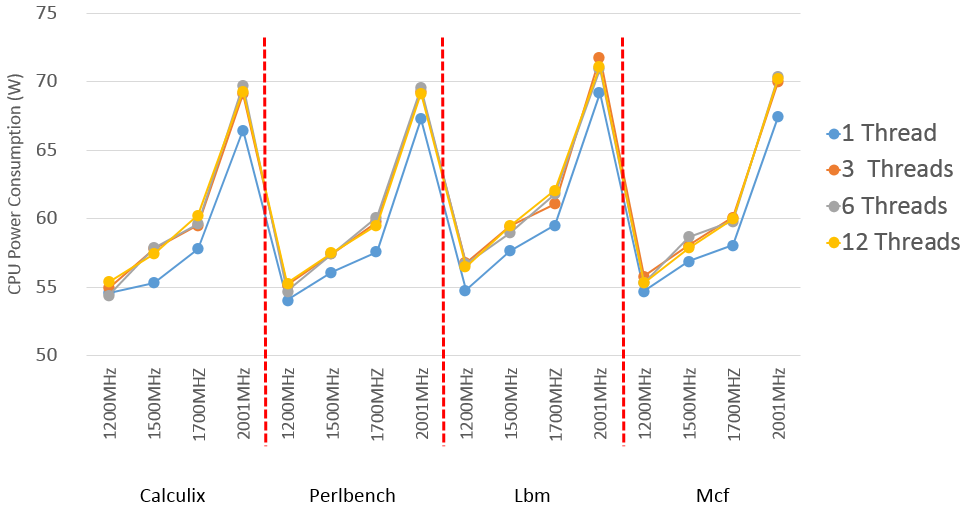
\includegraphics[scale= 0.6]{Screenshot_1} % Podría poner[width=\linewidth]
\caption{CPU power consumption depending on frequency and threads enabled}
\label{fig:powerProc} %Establece una etiqueta para la figura
\end{center}
\end{figure}

All the plots have the same shape. The "1 Thread Plot" has lower CPU power consumption. This reduction is not more than 4W which is the sensor resolution, so no assurance may be given.

This difference is because the total consumption of the server remains the same, but the consumption of fans and memories increases 1-2W. Figure \ref{fig:powerProcTotal} represents the total consumption of the server which we can see that is the same for any number of threads enabled.

\begin{figure}[H]
\begin{center}
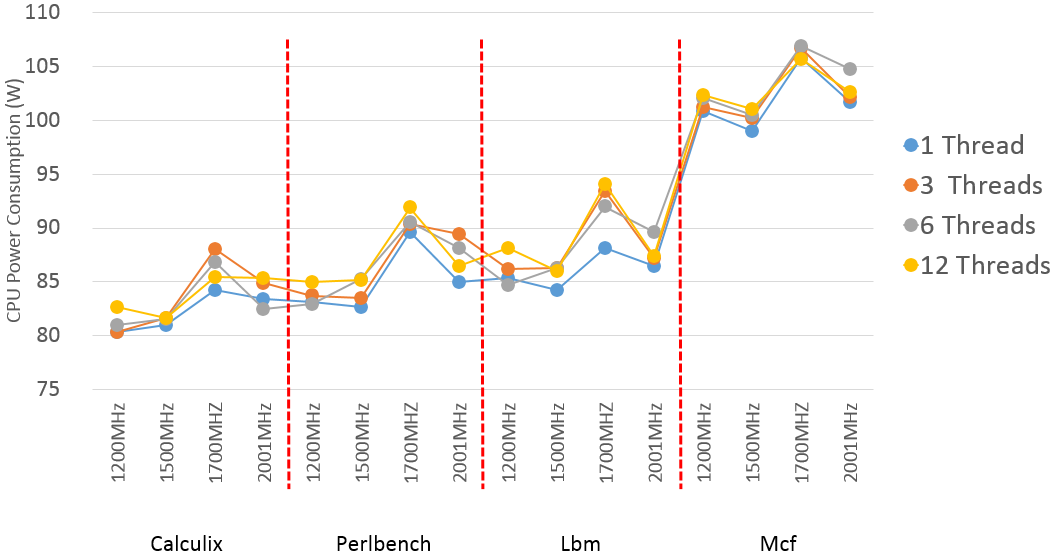
\includegraphics[scale= 0.6]{Screenshot_2} % Podría poner[width=\linewidth]
\caption{Total power consumption depending on frequency and Threads enabled}
\label{fig:powerProcTotal} %Establece una etiqueta para la figura
\end{center}
\end{figure}

Finally, all this study would have given more results if intel-pstate driver was enabled to be configured by the user. The newest Intel servers have this driver that allows the OS to manage the number of cores that are turned on and off depending of the workload.

\subsection{Analysis of tentative policies}

In this section, a comparison between DVFS and disabling threads will be given. The point is to study which actuation technique is better to apply when consumption reduction is needed.

First of all, if the need is to achieve a peak power consumption reduction, given that disabling threads does not reduce the power consumption, the only way is reducing the frequency of the processor. Reducing the frequency, the processor computes slower and consumes less power. Figure \ref{fig:compPower} represents the CPU total consumption depending on the frequency.

\begin{figure}[H]
\begin{center}
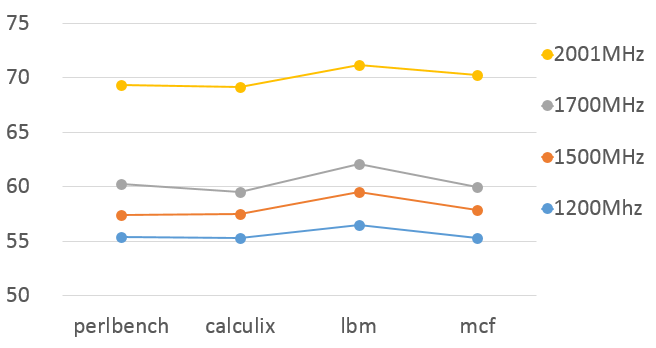
\includegraphics[scale= 0.7]{compPower2} % Podría poner[width=\linewidth]
\caption{CPU power consumption depending on frequency}
\label{fig:compPower} %Establece una etiqueta para la figura
\end{center}
\end{figure}


When energy consumption reduction is the aim, the choice is not as simple as power. We have two actuation techniques that are orthogonal between them and the best solution is not just incrementing one of them. Table \ref{tab:energComp} is an example of the consumption of a benchmark - perlbench - depending on the frequency and the number of threads enabled. Despite this table shows a particular example, this reasoning can be applied to all benchmarks.

\begin{table}[H]
\begin{center}
\begin{tabular}{ccccc}
  \bf Perlbench &  1200MHz & 1500MHz & 1700MHz & 2001MHz \\
  \bf 1 Thread &  7.5 $\cdot {10}^{4}$ & 5.6 $\cdot {10}^{4}$ & 5.1 $\cdot {10}^{4}$ & 3.6 $\cdot {10}^{4}$ \\
  \bf 3 Threads & 5.3 $\cdot {10}^{4}$ & 4.5 $\cdot {10}^{4}$ & 4.1 $\cdot {10}^{4}$ & 3.2 $\cdot {10}^{4}$ \\
  \bf 6 Threads & 5.3 $\cdot {10}^{4}$ & 4.4 $\cdot {10}^{4}$ & 4.0 $\cdot {10}^{4}$ & 3.3 $\cdot {10}^{4}$ \\
  \bf 12 Threads & 5.4 $\cdot {10}^{4}$ & 4.4 $\cdot {10}^{4}$ & 4.1 $\cdot {10}^{4}$ & 3.3 $\cdot {10}^{4}$ \\

\end{tabular}
\end{center}
\caption{CPU energy consumption of 1 copy of Perlbench depending on Frequency and number of threads enabled }
\label{tab:energComp}
\end{table}

As it can be seen in the table, if we are executing one copy of Perlbench with just one core and 1200Mhz, and we need to reduce the energy consumed, the first step would be increasing the number of threads enabled for this benchmark to 3 threads.

Then there is no more reduction for enabling more threads - this is because more than 2 threads does not reduce the time elapsed. Now, it would be necessary to increase the frequency using DVFS.

Increasing frequency reduces energy consumption, but it should be the opposite. This is because we are always using the Total CPU Consumption data. This data contains the contribution of the IDLE consumption, which is large and constant, and it is calculated depending on the time elapsed in the benchmark. 

When only the dynamic CPU power consumption is compared, energy consumption has a growth of consumption trend with the frequency. The issue is that the power measured is lower than the sensor resolution, so values are just indicative. 
%\begin{comment}
Table \ref{tab:energCompdyn} shows this information for the same benchmark.

\begin{table}[H]
\begin{center}
\begin{tabular}{ccccc}
  \bf Perlbench &  1200MHz & 1500MHz & 1700MHz & 2001MHz \\
  \bf 1 Thread &  2.7 $\cdot {10}^{3}$ & 1.7 $\cdot {10}^{3}$ & 3.7 $\cdot {10}^{3}$ & 5.4 $\cdot {10}^{3}$ \\
  \bf 3 Threads &  1.2 $\cdot {10}^{3}$ & 2.8 $\cdot {10}^{3}$ & 4.1 $\cdot {10}^{3}$ & 5.6 $\cdot {10}^{3}$ \\
  \bf 6 Threads & 2.9 $\cdot {10}^{3}$ & 3.1 $\cdot {10}^{3}$ & 3.8 $\cdot {10}^{3}$ & 5.8 $\cdot {10}^{3}$ \\
  \bf 12 Threads &  2.6 $\cdot {10}^{3}$ & 2.7 $\cdot {10}^{3}$ & 4.7 $\cdot {10}^{3}$ & 5.9 $\cdot {10}^{3}$ \\

\end{tabular}
\end{center}
\caption{Dynamic CPU energy consumption of 1 copy of Perlbench depending on Frequency and number of threads enabled }
\label{tab:energCompdyn}
\end{table}
%\end{comment}

These are the results that have been obtained from the study of the Decathlete server in this thesis. In the next chapter, the most important conclusions and the proposed future lines of work will be detailed.
\chapter{Conclusions}

Nowadays, reducing the power consumption and therefore costs is one of the main goals of any business. Specially in data centers, where the largest item of expenditure is the power cost, it is a critical goal.

In this thesis, the main objective has been analyzing all non-intrusive actuation control techniques for enterprise servers, focusing in the OCP Decathlete in order to provide support to the optimization of researches. This server has been chosen due to it is open design and all the customization possibilities this involves.

First, it has been analyzed how to change the configuration of memories, processors and fans in several ways. Then, the second phase had the aim of managing them at user space level in the OS. This would generalise this new technique for as many server models as possible helping the GreenLSI to implement it in all their servers.

For those servers that can be currently controlled, some benchmarks have been tested in order to model the behaviour of the server using different power configurations. Thanks to the results of the benchmarks, the relation between the power consumption and the performance has been quantified.

Finally, it has been studied the implications of using DVFS or turning off some CPUs in each type of workload in order to define a new saving policy to apply in the server.

\newpage
\section{Future Work}

Here I will list the main points I think future works should be focused in order to achieve the goal of controlling this enterprise server.

\emph{Future actions on actuation techniques}

\begin{itemize}

\item Firstly, it is important to rise the actuation level of some subsystems, specially fans control which can only be managed using the SP, to the OS level. This effort will help the GreenLSI to control the fan speed as they want to be able to create solid actuation policies.

\item During this project we analyzed the firmware deployed at the SP and we believe it would be possible to add support at the firmware level for fan control.



\emph{Research items}

\item At the end of this thesis we have provided a way to enable and disable memory DIMMs. However, a deep assessment on the power/energy/EDP benefits of this approach needs to be investigated. Moreover, this open new research challenges from the workload allocation perspective, allowing to decide the amounts of DIMMs active for each workload.

\item Finally, now that it is known how it affects to the server the DVFS and the CPU's off, it is necessary to create a complex policy based on the different type of workloads - CPU intensive and Memory intensive - in order to save the maximum amount of energy as possible combining those techniques.
\end{itemize}


\cleardoublepage
 \backmatter
\nocite{*}
\bibliographystyle{unsrt} %unsrt %plainurl %ieeetr
\bibliography{References}
\addcontentsline{toc}{part}{References}

%\input{References}

\printindex

\cleardoublepage
\newpage
\vspace*{13cm}

%\hline

\begin{center}
This page is left blank intentionally.
\end{center}
\end{document}